\section{Related work\label{sec:relwork}}
This chapter presents the techniques and conclusions of the literature review. Firstly, an analysis will be made of the research already carried out on our subject. The methodology and reasoning behind the literature review will be presented, together with a summary of the results. Next, a comparison of current tools that are close to the objective of this thesis will be carried out.\\

    \subsection{State of the Art}
        \subsubsection{\acrfull{sms}}
        Systematic mapping is a strategy for creating a categorization system and organizing a specific topic of interest \cite{petersen2008systematic}. It is a research approach that involves examining current published research reports, evaluating them in depth and summarizing their methodology and conclusions. It is carried out in several stages, as shown in the Figure\ref{fig:SysMapProcess}, and results in a classification (mapping) of the articles studied.\\

        \begin{figure}[h]
            \centering
            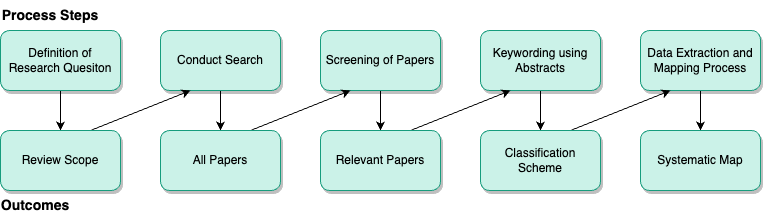
\includegraphics[scale=0.6]{images/RelatedWork-SysMapProcess.drawio.png}
            \caption{\label{fig:SysMapProcess}  The Systematic Mapping Process (Petersen et al. 2008) \cite{petersen2008systematic}}
        \end{figure}

        First, the \textbf{\acrshort{sms}} research questions had to be identified, which enabled a preliminary search for relevant articles to be carried out. These research questions should be considered as sub-questions of those defined in Section\ref{subsec:reseques}. The information extracted from these articles was used to develop a set of keywords and a categorization system. Before examining the articles to determine their relevance to this work, the inclusion, and exclusion criteria must be established. On the basis of the results, the context, and aspect of the research were defined. The final stage is the data extraction and mapping procedure, which results in a systematic map \cite{petersen2008systematic, petersen2015guidelines}.\\

            \paragraph{Research questions\label{para:res-ques}}
            The research questions defined in Section\ref{subsec:reseques} provide a more concise definition of the issues raised by the subject of this thesis. However, in order to learn from existing methodologies and possibly adapt elements of their tool chain, we need to ask more specific questions in the context of our \acrshort{sms}. To demonstrate the relationship with our main research questions, these are repeated and for each one a corresponding structured mapping study question (\textbf{SMS\_Q}) is presented.

            \begin{itemize}
                \item Q1: What are the main challenges and limitations of current configuration processes for simulations in the automotive industry?
                    \begin{itemize}
                        \item \textbf{SMS\_Q1}: What are the most frequently cited challenges associated with current configuration practices for simulations in the automotive industry?
                    \end{itemize}


                \item Q2: How can semantic technology be used to support simulation configuration processes?
                    \begin{itemize}
                        \item \textbf{SMS\_Q2}: What are the key concepts and principles of semantic technology that can be applied to simulation configuration?

                        \item \textbf{SMS\_Q3}: How can semantic technologies enable the representation and management of simulation configuration knowledge in a structured and machine-interpretable way?
                    \end{itemize}
                    
                \item Q3: What are the requirements of a semantic-based configuration tool for automotive simulations?
                    \begin{itemize}
                        \item \textbf{SMS\_Q4}: What are the essential functionalities and features that a semantic-based configuration tool for automotive simulations should possess?
                    \end{itemize}


                \item Q4: What are the existing semantic technologies and standards applicable to the field of systems engineering and simulation configuration, and how can they be adapted to support simulation configuration processes?
                    \begin{itemize}
                        \item \textbf{SMS\_Q5}: What are the prominent semantic technologies and standards that are relevant to systems engineering and simulation configuration?

                        \item \textbf{SMS\_Q6}: In what ways can these exist semantic technologies and standards be adapted or integrated to effectively support simulation configuration processes in the automotive industry?
                    \end{itemize}

            \end{itemize}

            
            \paragraph{Search strings for search}
            The Table\ref{tab:keyw-syno} shows the keywords obtained after the preliminary search.\\

            \begin{table}[h]
                \centering
        	    {\rowcolors{2}{teal!10}{white}
        	    \begin{tabular}{ | m{5.5cm} | m{9cm} | }
                    \hline
                    \rowcolor{teal!30} Keywords & Synonyms \\
                    
                    \hline
                    semantic technologies  & Ontologies, Knowledge graphs\\
                    
                    \hline
                    simulation data & Simulation knowledge\\
                    
                    \hline
                    Case-Based Reasoning  & Similarity-Based, Experience-Based, knowledge-Based Reasoning\\
                    
                    \hline
                    Rule-Based Reasoning  & \\
                    
                    \hline
                    Expert-System  & \\
                    
                    \hline
                    Computer Aided Engineering  & Computer Assisted Engineering\\
                    
                    \hline
                \end{tabular}}
                \caption{\label{tab:keyw-syno} Keywords and their synonyms}
            \end{table}

            The keywords found were then searched for synonyms, related phrases and alternative spellings \cite{budgen2006performing}. As usual, Boolean logic was used to define a search string, combining alternative phrases with \textbf{“OR”} and linking terms with \textbf{“AND”}. The final search string is as follows:

            \begin{lstlisting}[language=XML, caption=Generated Query, label={lst:gen-query}]
"semantic technologies" 
OR ("Ontology" AND "Simulation")
OR ("simulation configuration process" OR "simulation configuration workflow" OR "simulation configuration knowledge")
OR (("Case-Based Reasoning" OR "Similarity-Based Reasoning" OR "Experience-Based Reasoning" OR "knowledge-Based Reasoning") AND "Simulation")
OR ("Rule-Based Reasoning" AND "Simulation")
OR ("Expert-System" AND "Simulation")
OR (("Computer Aided" OR "Computer Assisted") AND "engineering")
            \end{lstlisting}

            Once the search query was obtained, the search was carried out in 3 main platforms: \textbf{ACM}, \textbf{IEEE} and \textbf{ScienceDirect}. 


            \paragraph{Inclusion and Exclusion Criteria}
            In this section, the inclusion, and exclusion criteria will be defined. They allow certain restrictions to be imposed in order to obtain only useful and relevant results.

            \begin{itemize}
                \item Inclusion criteria:
                    \begin{itemize}
                        \item \textbf{IC2}: Papers with keywords that match our query (at the level of their title or abstract).
                    \end{itemize}

                \item Exclusion criteria:
                    \begin{itemize}
                        \item \textbf{EC1} : Papers whose abstract content does not focus on one of the following themes:
                            \begin{itemize}
                                \item semantic technologies,
                                \item expertise systems
                                \item case-based reasoning
                                \item rule-based reasoning
                            \end{itemize}

                        \item \textbf{EC2} : Papers not written in English or German

                        \item \textbf{EC3} : Papers not publicly accessible from the chosen platforms
                    \end{itemize}
            \end{itemize}

            One point to emphasize is that in most mapping studies, an exclusion criterion is also defined in relation to the date of publication. This makes it possible to limit the period of publication of the results (e.g., 2002 — now). But this thesis revolves very much around case-based and rule-based reasoning, which are very old artificial intelligence techniques compared with modern methods.

            
            \paragraph{Classification Scheme}
            In this section, we follow the approach introduced by Bailey \cite{hill2019systematic} and described in Figure\ref{fig:BuildClassSchem}. Here, classification is based mainly on \textbf{keywording}. Keywording is a method of speeding up the classification process by extracting keywords from the abstracts of selected articles \cite{petersen2008systematic}. In this way, the context of each contribution can be easily obtained. Once this stage has been completed, an examination of the relevant keywords in each article provides an in-depth understanding of the nature and importance of the research \cite{petersen2008systematic}. \\
            This knowledge is used to create categories to classify all the articles. When the quality of abstracts is insufficient to allow the selection of significant keywords, it may be necessary to read the introduction and conclusion of an article.

            \begin{figure}[h]
                \centering
                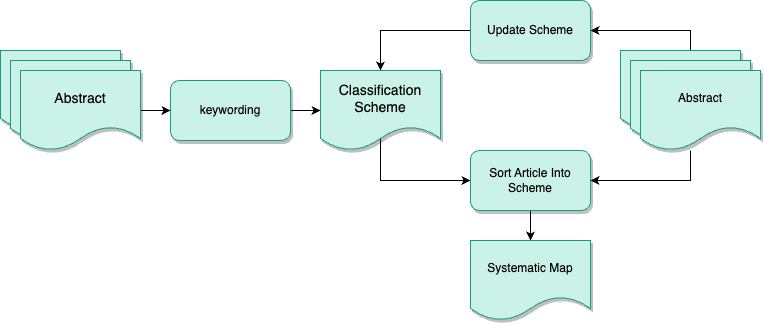
\includegraphics[scale=0.6]{images/RelatedWork-Build-Class-Schem.drawio.png}  \caption{\label{fig:BuildClassSchem}  Building the Classification Scheme \cite{petersen2008systematic}}
            \end{figure}

           In the context of this research, three facets have been identified. The first facet summarizes the subject of our thesis (i.e., Semantic Technologies usage). Table\ref{tab:sem-tec-usage} shows the possible values of this facet. The other two facets are more commonly used to group research contributions and can therefore be integrated \cite{petersen2008systematic, wieringa2006requirements}: research type and contribution.\\
            The research facet represents the research technique used in the study; these approaches are domain-neutral and can be used without change (Table\ref{tab:contri-ty-face}).\\
            The third facet, the contribution facet, documents the contribution made in terms of, for example, process, method or tool, etc. (Table\ref{tab:research-ty-face}).\\
            The results of the SMS are presented below. The appendix contains the full results.

        
            \begin{table}[h]
                \centering
        	    {\rowcolors{2}{teal!10}{white}
        	    \begin{tabular}{ | m{14.5cm} | }
                    \hline
                    \rowcolor{teal!30} Category \\
                    
                    \hline
                    Case-based reasoning\\
                    
                    \hline
                    Rule-based reasoning\\
                    
                    \hline
                    Expertsystem\\
                    
                    \hline
                    Knowledge representation\\
                    
                    \hline
                \end{tabular}}
                \caption{\label{tab:sem-tec-usage} Semantic Technologies usage}
            \end{table}

            \begin{table}[h]
                \centering
        	    {\rowcolors{2}{teal!10}{white}
        	    \begin{tabular}{ | m{2cm} | m{12.5cm} | }
                    \hline
                    \rowcolor{teal!30} Category & Description \\
                    
                    \hline
                    Metric  & Papers classified under Metric contributions focus on the creation or evaluation of specific measurement criteria or metrics within a certain context.\\
                    
                    \hline
                    Tool & Papers classified under Tool contributions describe the development, improvement, or assessment of software tools meant to meet specific difficulties in a certain domain.\\
                    
                    \hline
                    Model  & Papers in the Model contribution category contribute to the creation or enhancement of conceptual or computational models in a given topic.\\
                    
                    \hline
                    Method  & Method contributions concentrate on the development, improvement, or assessment of new research methodology or approaches.\\
                    
                    \hline
                    Process  & Papers in the Process contribution category focus on the design, assessment, or improvement of specific processes or workflows.\\
                    
                    \hline
                \end{tabular}}
                \caption{\label{tab:contri-ty-face} Contribution Type Facet}
            \end{table}

            \begin{table}[h]
                \centering
        	    {\rowcolors{2}{teal!10}{white}
        	    \begin{tabular}{ | m{2cm} | m{12.5cm} | }
                    \hline
                    \rowcolor{teal!30} Category & Description \\
                    
                    \hline
                    Validation Research  & The techniques explored are innovative and have not yet been used in practice. Experiments, or laboratory work, are one example of a technique employed.\\
                    
                    \hline
                    Evaluation Research & Techniques are put into practice, and their effectiveness is evaluated. That is, it is demonstrated how the approach is applied in practice (solution implementation) and what the implications are in terms of advantages and downsides (implementation assessment). This involves identifying difficulties in the industry.\\
                    
                    \hline
                    Solution Proposal  & A solution to a problem is given; the solution may be unique or a major expansion of an existing approach. A tiny example or a strong line of reasoning demonstrates the solution's potential benefits and application.\\
                    
                    \hline
                    Philosophical Papers  & These publications provide a new way of looking at existing objects by arranging the area in the form of a taxonomy or conceptual framework.\\
                    
                    \hline
                    Opinion Papers  & These articles offer the author's own view on whether a particular approach is excellent or terrible, or how things should have been done. They do not rely on previous work or research methods.\\
                    
                    \hline
                    Experience Papers  & Experience papers describe what and how something was done in practice. It must be based on the author's real experiences.\\
                    
                    \hline
                \end{tabular}}
                \caption{\label{tab:research-ty-face} Research Type Facet}
            \end{table}

    
        \subsubsection{Result}
        This section presents the results of the mapping study. Paragraph\ref{para:sms_analysis} provides an analysis of the results obtained, followed by in-depth answers to the research questions defined in Paragraph\ref{para:sms_ans_rq}.

            \paragraph{Results of Database Search}
            The predefined keywords and the EC2 criterion were used to obtain a total of 26270 research publications. These are classified as, 25175 for IEEE, 203 for ACM and 892 for ScienceDirect. Due to the EC3 exclusion criterion, the number of articles obtained fell to 389 for IEEE, 203 for ACM and 125 for ScienceDirect. For a total of 717 articles. The EC1 exclusion criterion was then used to reduce the number of relevant articles even further. This resulted in a total of 24 articles.\\
            This was followed by a manual keyword-by-keyword search, which produced better quality results. Manual target searching has been shown to produce high quality search results when combined with searches of digital libraries (Jorgensen and Shepperd 2007). We integrated manual target searches from other platforms, such as Google Scholar. This resulted in 27 additional articles. Table\ref{tab:rel-papers} shows the list of articles selected, classified by publication date. This list was filtered on the basis of inclusion and exclusion criteria, and duplicate articles from different platforms were removed.\\

            
        	    {\rowcolors{2}{teal!10}{white}
        	    \begin{longtable}{ | m{1cm} | m{1.5cm} | m{12cm} | }
                    \caption{\label{tab:rel-papers} Relevant papers, ordered by year of appearance}\\
                    \hline
                    \textbf{ID} &\textbf{Year} &\textbf{Title} \\
                    \hline
                    \endfirsthead
                    
                    \hline
                    \textbf{A28} &1992 &Fallbasiertes Schließen \cite{althoff1992fallbasiertes} \\
                    \hline
                    \textbf{A17} &1995 &Case based reasoning \cite{richter2016case} \\
                    \hline
                    \textbf{A26} &1995 &Fallbasiertes Schließen zur Kreditwürdigkeitsprüfung \cite{wilke1995fallbasiertes} \\
                    \hline
                    \textbf{A19} &2001 &A Tutorial on Case Based Reasoning \cite{main2001tutorial} \\
                    \hline
                    \textbf{A5} &2002 &Ontology-Driven Induction of Decision Trees at Multiple Levels of Abstraction \cite{zhang2002ontology} \\
                    \hline
                    \textbf{A18} &2003 &R5 model for case-based reasoning \cite{finnie2003r5} \\
                    \hline
                    \textbf{A20} &2003 &From Case-based Reasoning to Problem-based Learning \cite{eshach2003case} \\
                    \hline
                    \textbf{A3} &2006 &Using Ontologies for Simulation Modeling \cite{benjamin2006using}\\
                    \hline
                    \textbf{A30} &2007 &Using ontologies for simulation integration \cite{benjamin2007using}\\
                    \hline
                    \textbf{A4} &2008 &SemTree: ontology-based decision tree algorithm for recommender systems \cite{bouza2008semtree} \\
                    \hline
                    \textbf{A31} &2008 &Clustering with case-based reasoning for wireless sensor network \cite{wang2008clustering} \\
                    \hline
                    \textbf{A12} &2010 &Ontology-Based Context Representation and Reasoning Using OWL and SWRL \cite{liu2010ontology} \\
                    \hline
                    \textbf{A25} &2010 &Problem Solving by Case-Based Reasoning \\
                    \hline
                    \textbf{A27} &2010 &Problem Solving by Case-Based Reasoning 2 \\
                    \hline
                    \textbf{A49} &2010 &Using ontologies for the federated simulation of critical infrastructures \cite{tofani2010using} \\
                    \hline
                    \textbf{A21} &2011 &Case-Based Reasoning Research and Development \cite{wiratunga2011case} \\
                    \hline
                    \textbf{A11} &2012 &A recommendation system based on domain ontology and SWRL for anti-diabetic drugs selection \\
                    \hline
                    \textbf{A6} &2013 &Ontology Enhancement through Inductive Decision Trees \cite{chen2012recommendation} \\
                    \hline
                    \textbf{A29} &2013 &Developing a real-time inference approach for rule-based reasoning systems \cite{qiao2013developing} \\
                    \hline
                    \textbf{A16} &2014 &The Collaborative Agile Knowledge Engine CAKE \cite{bergmann2014collaborative} \\
                    \hline
                    \textbf{A46} &2014 &Domain Ontologies Integration for Virtual Modelling and Simulation Environments \cite{smirnov2014domain} \\
                    \hline
                    \textbf{A48} &2014 &An Ontology Framework for Rule-based Inspection of eeBIM-systems \cite{kadolsky2014ontology}\\
                    \hline
                    \textbf{A50} &2014 &Hybrid Fuzzy-ontological Project Framework of a Team Work Simulation System \cite{orlowski2014hybrid} \\
                    \hline
                    \textbf{A52} &2014 &Human System Integration Ontology: Enhancing Model Based Systems Engineering to Evaluate Human-system Performance \cite{orellana2014human}\\
                    \hline
                    \textbf{A51} &2015 &Decision Support in Production Planning of Precast Concrete Slabs Based on Simulation and Learning from Examples \cite{konczak2015decision} \\
                    \hline
                    \textbf{A7} &2016 &Development of an ontology-based configuration management system \cite{na2016development}\\
                    \hline
                    \textbf{A9} &2016 &Automatic CAD model retrieval based on design documents using semantic processing and rule processing \cite{jeon2016automatic}\\
                    \hline
                    \textbf{A13} &2017 &Conversational Process-Oriented Case-Based Reasoning \cite{zeyen2017conversational}\\
                    \hline
                    \textbf{A34} &2017 &Case-Based Reasoning for Product Style Construction and Fuzzy Analytic Hierarchy Process Evaluation Modeling Using Consumers Linguistic Variables \cite{wang2017case}\\
                    \hline
                    \textbf{A45} &2017 &Development of Knowledge-Expandable Ontology-Based Expert System for Process Planning in Cold Forging of Flange Nuts \cite{chang2017development}\\
                    \hline
                    \textbf{A8} &2018 &An ontology-based product design framework for manufacturability verification and knowledge reuse \cite{li2018ontology}\\
                    \hline
                    \textbf{A10} &2018 &Improving integrated product design using SWRL rules expression and ontology-based reasoning \cite{abadi2018improving}\\
                    \hline
                    \textbf{A14} &2019 &ProCAKE: A Process-Oriented Case-Based Reasoning Framework \cite{bergmann2019procake}\\
                    \hline
                    \textbf{A22} &2019 &Modeling CBR using Python for Football Matches \cite{sawalkar2019modeling} \\
                    \hline
                    \textbf{A38} &2019 &An Adaptive Model for Identification of Influential Bloggers Based on Case-Based Reasoning Using Random Forest \cite{asim2019adaptive} \\
                    \hline
                    \textbf{A23} &2020 &A Simple Approach to Case-Based Reasoning in Knowledge Bases \cite{das2020simple} \\
                    \hline
                    \textbf{A32} &2020 &A Novel Case Base Reasoning and Frequent Pattern Based Decision Support System for Mitigating Software Risk Factors \cite{asif2020novel} \\
                    \hline
                    \textbf{A39} &2020 &A Novel Optimized Case-Based Reasoning Approach With K-Means Clustering and Genetic Algorithm for Predicting Multi-Class Workload Characterization in Autonomic Database and Data Warehouse System \cite{shaheen2020novel}\\
                    \hline
                    \textbf{A43} &2020 &A Similarity Measure in Formal Concept Analysis Containing General Semantic Information and Domain Information \cite{wang2020similarity} \\
                    \hline
                    \textbf{A2} &2021 &OSMO: Ontology for simulation, modelling, and optimization \cite{horsch2021osmo} \\
                    \hline
                    \textbf{A15} &2021 &Improving Similarity-Based Retrieval Efficiency by Using Graphic Processing Units in Case-Based Reasoning \cite{malburg2021improving} \\
                    \hline
                    \textbf{A35} &2021 &Exploiting Ontology Recommendation Using Text Categorization Approach \cite{sarwar2020exploiting} \\
                    \hline
                    \textbf{A36} &2021 &On Approximation of Concept Similarity Measure in Description Logic ELH With Pre-Trained Word Embedding \cite{racharak2021approximation}\\
                    \hline
                    \textbf{A37} &2021 &Semankey: A Semantics-Driven Approach for Querying RDF Repositories Using Keywords \cite{abad2021semankey} \\
                    \hline
                    \textbf{A40} &2021 &Multivariable Case Adaptation Method of Case-Based Reasoning Based on Multi-Case Clusters and Multi-Output Support Vector Machine for Equipment Maintenance Cost Prediction \cite{lin2021multivariable} \\
                    \hline
                    \textbf{A41} &2021 &Predicting Influential Blogger’s by a Novel, Hybrid and Optimized Case Based Reasoning Approach With Balanced Random Forest Using Imbalanced Data \cite{asim2020predicting}\\
                    \hline
                    \textbf{A47} &2021 &ORVIPO: An Ontological Prototype for Modeling 3D Scenes in Operating Rooms \cite{jaziri2021orvipo} \\
                    \hline
                    \textbf{A42} &2022 &F-CBR: An Architecture for Federated Case-Based Reasoning \cite{jaiswal2022f} \\
                    \hline
                    \textbf{A44} &2022 &An Interval Type-2 Fuzzy Ontological Similarity Measure \cite{adel2022interval} \\
                    \hline
                    \textbf{A1} &2023 &Simulation Data goes Ontology \cite{spelten2023simulation} \\
                    \hline
                    \textbf{A33} &2023 &A Generation and Repair Approach to Scheduling Semiconductor Packaging Facilities Using Case-Based Reasoning \cite{park2023generation} \\
                    \hline
                \end{longtable}}
            
            Here, a bubble chart has been used to present the frequencies, as shown in Figure\ref{fig:viz-smb}. Essentially, these are two x-y scatter plots whose bubbles represent category crossovers. The size of a bubble is proportional to the number of items in the category pair corresponding to its coordinates. The same concept is repeated, in separate quadrants of the same figure, to demonstrate the intersection with the third aspect. In the case of this thesis, bubble charts are more useful for analysis than frequency tables. It is simpler to evaluate many facets at once, although summary data can still be provided for specific facets. It's also more effective at providing a quick overview of a domain, thus acting as a map. In addition to this diagram, Figure\ref{fig:distro-art} presents sector diagrams showing the statistical distribution of each of our facet points.

            
            \begin{figure}[h]
            \centering
            \bubbleplot[%
                width=1cm,
                height=1cm,
                xmin=-7,
                xmax=8,
                ylabel="Semantic Technologies usage",
                meta=nbr,
                x field=x,
                enlarge y limits=0.3,
                x index field=ix,
                y field=y,
                y index field=iy,
                year field=years,
                year x shift=1cm,
                year y shift=0cm,
                year padding=0,
                x left label="Contribution Type Facet",
                x left label shift=4cm,
                x right label="Research Type Facet",
                x right label shift=0cm,
            ]{assets/MappingStud.csv}{1992, 1995, 2001, 2002, 2003, 2006, 2007, 2008, 2010, 2011, 2012, 2013, 2014, 2015, 2016, 2017, 2018, 2019, 2020, 2021, 2022, 2023}
            \caption{\label{fig:viz-smb}  Visualization of a Systematic Map as a Bubble Plot (each color represent different years of publication)}
            \end{figure}

            \begin{figure}[h]
                \centering
                \begin{subfigure}[b]{0.45\textwidth}
                    \centering
                    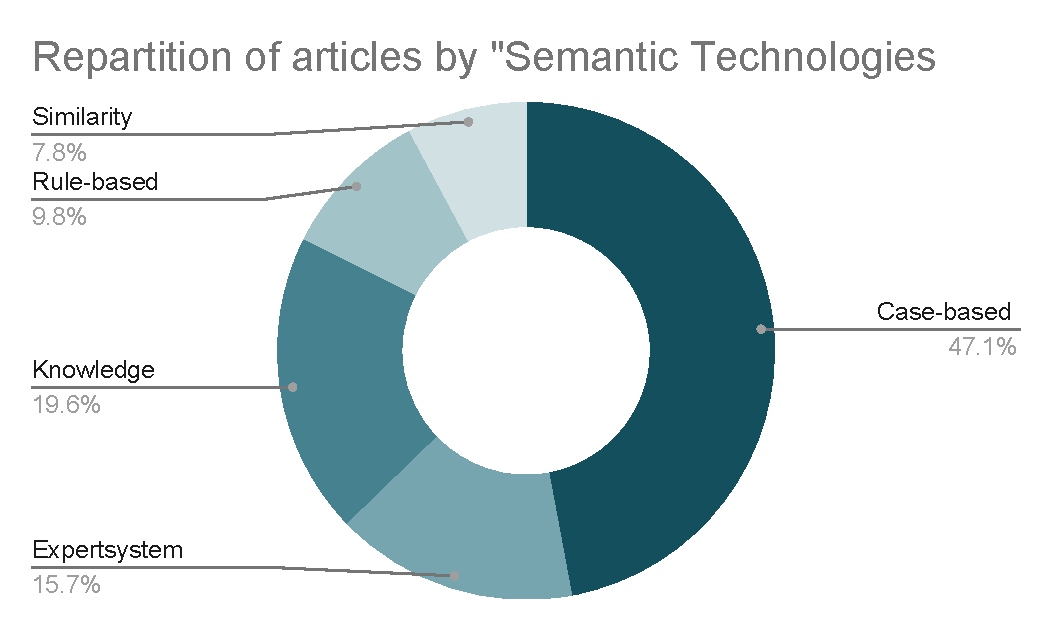
\includegraphics[width=\textwidth]{images/Repartition_by_Semantic_Technologies_usage.pdf}
                \end{subfigure}
                \begin{subfigure}[b]{0.45\textwidth}
                    \centering
                    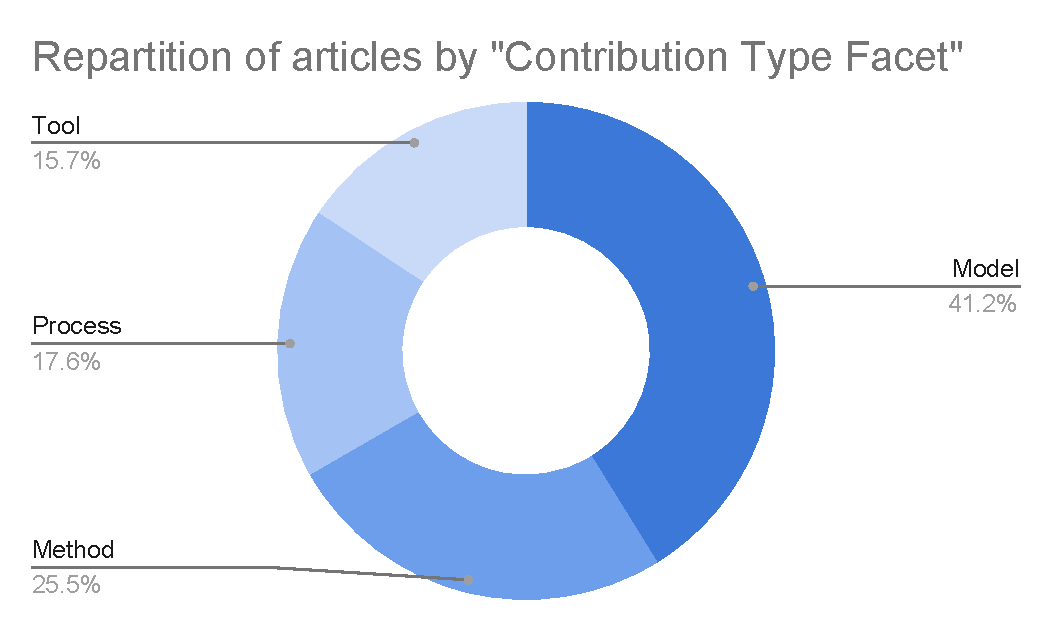
\includegraphics[width=\textwidth]{images/Repartition_by_Contribution_Type_Facet.pdf}
                \end{subfigure}
                \begin{subfigure}[b]{0.45\textwidth}
                    \centering
                    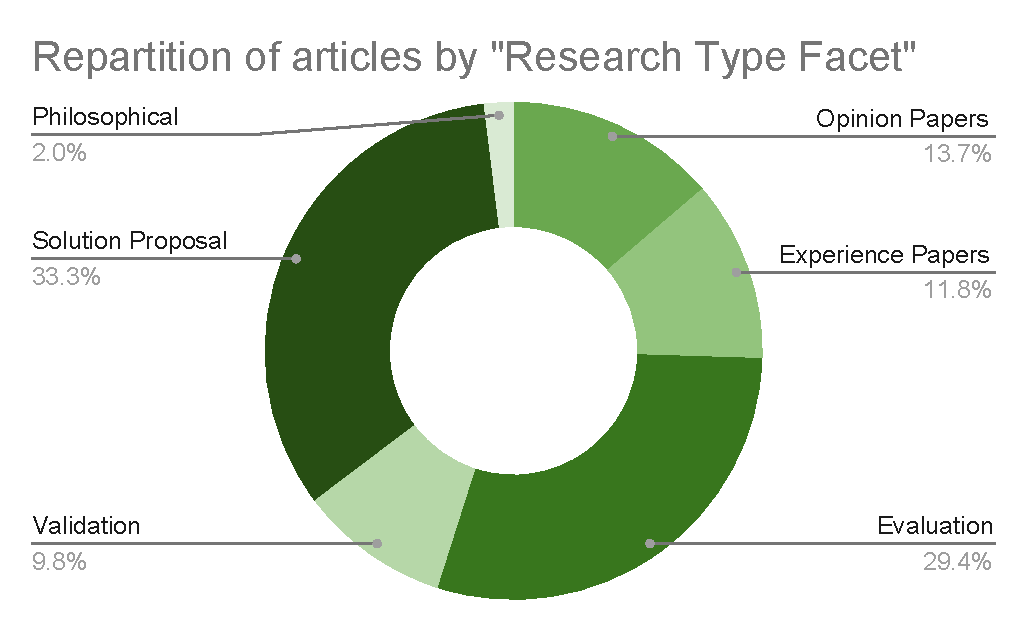
\includegraphics[width=\textwidth]{images/Repartition_by _Research_Type_Facet.pdf}
                \end{subfigure}
                \caption{\label{fig:distro-art} Distributions of the articles}
            \end{figure}
            
            \paragraph{Analysis\label{para:sms_analysis}}
            The mapping study shows that the use of semantic technologies in engineering goes back many years. In particular, these technologies are used to represent concepts and knowledge, and to set up expertise systems. These systems can be based on rule-based or case-based reasoning.\\
            
            In terms of type of contribution, the vast majority of articles found (41.5\%) were models. This shows that the use of semantic technologies in systems engineering remains largely experimental. Numerous authors propose ideas for integrations that could more or less work \cite{benjamin2007using, tofani2010using, benjamin2006using, bouza2008semtree}. 25.5\% and 17.6\% represent the percentage of articles on Methods and Processes, respectively. In the them, authors describe and evaluate solutions to specific problems. Only 15.7\% of articles are dedicated to tools. This shows that very little software exists for the creation and integration of semantic technologies in engineering.\\
            As far as the type of research is concerned, 33.3\% of the articles focus on solution proposals and 29.4\% on research evaluations. In other words, each paper was prepared as part of a project addressing a specific problem. A remedy was then proposed, and usually a small case study was studied. This demonstrates the popularity of these technologies with researchers. But from the other statistics it can be concluded that their use is still in the testing phase and their adoption is still timid.\\

            The next step in our analysis is to interpret the figures according to how semantic technologies are used.\\
            Starting with knowledge representation, there are few tools in use. As presented in [ , , ], the tool generally used to create or maintain ontologies is “Protégé”. There is no procedure for setting up these ontologies [ ]. This is why very few articles are based on a step-by-step presentation of the process. The team behind “Protégé” has nevertheless put together a set of best practices to follow [ ] in order to work as optimally as possible with their software. There are, however, articles that show how to create an ontology and the steps to follow [ , , ], but these are mostly domain-specific. \\

            When creating an ontology, it is possible to define constraints and rules that will be used by reasoners to perform inferences [ , , ]. These rules can be further defined using SWRL (Semantic Web Rule Language) [ ]. This ontological language is based on OWL and, thanks to the principle of FOL (First Order Logic), allows conditions to be defined, as well as the result if they are verified or not [ ]. A number of tools, such as JavaDON [] or the "SWRLTab" plugin for “Protégé” [], make it easy to define these rules. As demonstrated in [ , , ], the process of creating these rules is fairly standard and requires only a deep understanding of the relationships and interdependencies between the various elements of the ontology.\\

            Alongside rule-based reasoning, there is also case-based reasoning. The latter is used in the field of artificial intelligence [ ], but is becoming less and less popular, being replaced by deep learning and neural networks [ ]. In the field of engineering, there are numerous model proposals and experimental procedures [ , , ], which show how this reasoning could be used to solve specific problems. Nevertheless, it remains very popular with companies for assisting employees in making decisions based on previous decisions present in archives [ ]. Compared with other AI techniques, CBR considerably reduces the work involved in gathering and representing knowledge, which is undoubtedly one of the main reasons for the commercial success of CBR applications [ ]. Tools for performing case-based reasoning are few and fairly old [ ]. They include ProCake, myCBR, jCOLIBRI and others.\\

            When it comes to case-based reasoning, much of the research focuses on how similarity values between elements can be calculated. As shown in the articles [, ,] there are numerous algorithms for calculating similarity between values depending on their type. In particular, these algorithms are used in case-based reasoning, as shown in [ ].\\

            Both rules- and case-based reasoning are integrated into expertise systems []. As presented in Section\ref{subsec:exp-sys}, these systems support users in carrying out specific tasks based on the knowledge provided by experts. The basic architecture of how these systems are structured is fairly straightforward, but their implementation is generally company-specific [ ]. Tools such as JavaDON [ ] or Jess [ ] propose procedures to follow in order to set up such tools. Unfortunately, these studies were carried out many years ago, and the tools presented are no longer really maintained and updated.\\

            To sum up, semantic technologies are used in a variety of fields, including engineering. The ontologies they define enable the creation of data graphs that can be understood by machines (reasoning). They can also be used to define rules about the relationships and properties of elements present in the graph. These rules can be used for inference and reasoning. Another use for ontologies is case-based reasoning. Information from previous cases (data on the configurations of simulations carried out in the past) can be represented in an ontology, and thanks to the particularities of ontologies, a similarity calculation can be carried out to propose possible solutions to users. Both of these approaches have been successful in the professional world, but are unfortunately increasingly being replaced by artificial intelligence and modern methods such as deep learning and decision trees.\\

            
            \paragraph{Answering research questions\label{para:sms_ans_rq}}
            The primary aim of this mapping study is to identify research gaps, provide an overview of the approaches employed, and outline what can be expected from the use of the aforementioned tools. The answers to the questions defined in Section\ref{para:res-ques} are as follows.\\

            \textbf{SMS\_Q1}: What are the most frequently cited challenges associated with current simulation configuration practices in the automotive industry?
            \begin{quote}
                There are many challenges to highlight in the various collected articles related to simulation. The most common being:

                \begin{itemize}
                    \item \textbf{The complexity} [ , , ] : Modern systems are increasingly complex, with many interacting components. Setting up simulations for large-scale systems can be difficult due to the sheer number of variables, dependencies, and interactions involved. This leads to concerns about traceability. Individual configuration changes can often have a significant influence on overall system performance, complicating troubleshooting and analysis.
                    \item \textbf{The standardization} [ , , ] : The absence of standardized simulation procedures and formats, units and naming standards between different tools and teams poses compatibility problems and makes it difficult to share simulations.
                    \item \textbf{Lengthy setup times} [ , , ]: Setting up simulations often requires extensive manual configuration of tools and parameters, which is time-consuming, error-prone, and inconsistent.
                    \item \textbf{Limited reusability} [ , , ]: It can be difficult to develop simulation configurations that can be easily adapted to different circumstances and reused for several projects. It is essential to ensure that the configuration is flexible and that no major reworking is required for each use case.\\
                \end{itemize}
            \end{quote}

            \textbf{SMS\_Q2}: What are the key concepts and principles of semantic technology that can be applied to simulation configuration?
            \begin{quote}
                From the above problems, it is clear that the formalization of the elements and metadata of a simulation is a fairly critical point. It ensures collaboration between different players and the sustainability of previous simulations. This problem could be solved using ontologies [ ]. By setting up an ontology for simulations, it is possible to define standards for names and units of measurement. It is also possible to define the interdependent relationships between the various elements of simulations, the rules to be followed when assigning values to parameters, etc… Here, it is possible to apply the principles of case-based or rule-based reasoning presented in Section[].\\
            \end{quote}

            \textbf{SMS\_Q3}: How can semantic technologies enable the representation and management of simulation configuration knowledge in a structured and machine-interpretable manner?
            \begin{quote}
                As mentioned above, ontologies represent a promising means of standardization. By creating an ontology, a knowledge tree is established. To target the problems associated with the configuration process, the elements required to configure a simulation must first be integrated into the ontology. The next step is to define the possible attribute values of these elements, as well as their interdependent relationships.\\
            \end{quote}

            \textbf{SMS\_Q4}: What are the essential functionalities and features that a semantic-based configuration tool for automotive simulations should possess?
            \begin{quote}
                A semantics-based configuration tool for simulations should have certain capabilities and features critical to successfully solving the complicated simulation design problems discussed above. Ideally, such a tool should include the following crucial features:
                \begin{itemize}
                    \item \textbf{Data Management}: Use ontologies to specify the meaning and relationships between data, promoting consistency and understanding [ ].
                    \item \textbf{Semantic search and filtering}: Locate particular configuration items or variants using semantic attributes and connections [ ].
                    \item \textbf{Version control and branching}: manage multiple configuration versions while enabling comparison, rollback and merge [ ].
                    \item \textbf{Impact analysis}: Estimate the effects of modifications to individual configuration components on overall simulation results [ ].
                    \item \textbf{Version control with user access management}: Facilitate cooperation by controlling user access to different versions of the configuration.
                    \item \textbf{Annotation and documentation}: Allow users to annotate and record specific configuration choices and their justifications.
                    \item \textbf{Reusable configuration repository}: Templates let you save and distribute frequently used configurations for easy reuse.
                    \item \textbf{Integration with knowledge management systems}: connect to existing knowledge bases to document and share best practices and lessons learned.
                    \item \textbf{Scalability and performance}: manage complex parameters and large data sets efficiently.\\
                \end{itemize}
            \end{quote}

            \textbf{SMS\_Q5}: What are the prominent semantic technologies and standards that are relevant to systems engineering and simulation configuration?
            \begin{quote}
                Semantic technologies such as RDFS, OWL, SPARQL, and many others are therefore of crucial importance [].\\
            \end{quote}

            \textbf{SMS\_Q6}: In what ways can these existing semantic technologies and standards be adapted or integrated to effectively support simulation configuration processes in the automotive industry?
            \begin{quote}
                The integration of these technologies could be achieved by setting up an expert-system [ ]. This system could use knowledge from experts stored in an ontology. Then, thanks to rules defined in the ontology and case reasoning, the expertise system will be able to assist the user by means of an inference unit (reasoner).  Figure\ref{fig:es-archi} shows the architecture of an expertise system.\\
            \end{quote}
        
    \subsection{State of Practice}
        \subsubsection{Semantic Web Technologies\label{sec:semtec}}
        Semantic technology is a set of approaches, tools, and strategies that offer sophisticated mechanisms for enhancing data in a domain with explicit meanings, making it understandable to computers. By creating data models known as ontologies, semantic web technologies represent an area of interest with a high degree of abstraction.\\ 
        
            \paragraph{RDF's Serializations}
                Unlike other data models, RDF data models do not rely on a single serialization syntax. Triples in an RDF dataset can be serialized in a number of ways [], and some of the most common serialization methods are : 

                \begin{itemize}
                    \item \textbf{RDF/XML}: RDF/XML is the most widely used serialization format for RDF in the W3C recommendations. RDF/XML is an XML-style tree document with a graph based on triples, which makes it theoretically difficult and verbose. 
                    \item \textbf{Notation3 (.n3)}: Unlike R/XML, N3 syntax is more concise and easier to understand because it is closer to the subject-predicate-object paradigm of RDF. 
                    \item JSON for Linking Data (JSON-LD) is a relatively new, user-friendly format. It combines web syntax (JSON) with RDF principles. [ ] 
                    \item \textbf{Turtle}: The Turtle syntax is the successor to the N3 syntax, allowing more concise encoding of RDF data.
                \end{itemize}

                Listing \ref{lst:rdf-xml}, Listing \ref{lst:rdf-turtle} and Listing \ref{lst:rdf-json-ld} show the serializations of a single example in different formats (RDF/XML, Turtle, JSON-LD) and the Figure \ref{fig:rdf-xml-example} shows the graphical representation in RDF/XML. As you can see, the “turtle” syntax uses namespace prefixes to provide a more concise and clear syntax. It can also be used to describe lists of predicates or objects. There are also various serialization syntaxes for representing RDF. However, due to its short structure and readability, the “turtle” syntax is used in this thesis for ontology development.\\
            
                \begin{figure}[h]
                    \centering
                    
\includegraphics[scale=0.6]{images/Foundation-RDF XML.drawio.png}
                    \caption{\label{fig:rdf-xml-example}  Graph Example in RDF/XML}
                \end{figure}

                \begin{lstlisting}[language=XML, caption=Example of RDF Serialization in RDF/XML, label={lst:rdf-xml}]
<?xml version="1.0" encoding="utf-8" ?>
<rdf:RDF xmlns:rdf="http://www.w3.org/1999/02/22-rdf-syntax-ns#"
            xmlns:ns0="http://dbpedia.org/ontology/">

    <rdf:Description rdf:about="http://dbpedia.org/resource/Pluto">
        <ns0:discovered>1930</ns0:discovered>
        <ns0:discoverer rdf:resource="http://dbpedia.org/resource/Clyde_Tombaugh"/>
    </rdf:Description>
</rdf:RDF>
                \end{lstlisting}

                \begin{lstlisting}[caption=Example of RDF Serialization in Turtle, label={lst:rdf-turtle}]
@prefix ns0: <http://dbpedia.org/ontology/> .

<http://dbpedia.org/resource/Pluto>
  ns0:discovered "1930" ;
  ns0:discoverer <http://dbpedia.org/resource/Clyde_Tombaugh> .
                \end{lstlisting}

                \begin{lstlisting}[caption=Example of RDF Serialization in JSON-LD, label={lst:rdf-json-ld}]
[ {
  "@id" : "_:genid1",
  "@type" : [ "http://www.w3.org/2002/07/owl#Ontology" ]
}, {
  "@id" : "http://dbpedia.org/ontology/discovered",
  "@type" : [ "http://www.w3.org/2002/07/owl#AnnotationProperty" ]
}, {
  "@id" : "http://dbpedia.org/ontology/discoverer",
  "@type" : [ "http://www.w3.org/2002/07/owl#AnnotationProperty" ]
}, {
  "@id" : "http://dbpedia.org/resource/Pluto",
  "http://dbpedia.org/ontology/discovered" : [ {
    "@value" : "1930"
  } ],
  "http://dbpedia.org/ontology/discoverer" : [ {
    "@id" : "http://dbpedia.org/resource/Clyde_Tombaugh"
  } ]
} ]
                \end{lstlisting}

                
        
        
        

            \paragraph{Model Building with RDFS}
            RDFS presents the main techniques for creating a taxonomy and instantiating objects [ ] : 

            \begin{itemize}
                \item Subclass Statements : As in object-oriented programming, the rdfs:subClassOf statement allows an rdfs:Class to inherit the attributes and descriptions of its superclass while allowing further definition. rdfs:subPropertyOf works in the same way as rdf:Property. Unlike object-oriented programming, a class can be a subclass of more than one superclass. 
                \item Property domain and range: Properties can be defined using the attributes rdfs:domain and rdfs:range. They indicate that the subject or object of a triple containing the property must belong to the given classes. Multiple domain or range axioms must be read in combination. This means that if the domain has several limits, the object of the triple must satisfy both axioms. 
                \item Instantiating an object: \textbf{rdf:type} creates an object as an instance of a \textbf{rdfs:Class}. This is often abbreviated to “$is\_a$” or “a”. [ ] 
            \end{itemize}
    
            \paragraph{OWL}
            The W3C group created the OWL language as a set of formal languages for semantic ontologies on the Web []. OWL shares many properties with RDF; in fact, it is an extension of the RDF vocabulary []. An OWL ontology is represented by an RDF graph. It can be serialized using one of the RDF syntaxes described above. \\
        
            An OWL ontology includes an optional ontology header, class axioms, property axioms and information about individuals/instances. The OWL vocabulary is derived from the OWL namespace: "$https://www.w3.org/2002/07/owl\#$". 
        
            \begin{itemize}
                \item Instance: An instance is the equivalent of an object in object-oriented modelling. 
                \item Class: A class is a collection of elements. A class can contain any number of instances. A class in an OWL ontology can be a subclass of another class, inheriting the characteristics of the parent class. All classes are considered subclasses of the owl:Thing class, which is the root class of an OWL ontology and represents the collection of all people. 
                \item Object properties : The properties that link people (instances) of two OWL classes. All object properties are subclasses of owl:ObjectProperty. 
                \item Data type attributes: These attributes link people (instances) of OWL classes to literal values. All datatype properties are subclasses of owl:DatatypeProperty.
            \end{itemize}
        
            OWL is made up of structures and terminology used to semantically represent a domain. It is a set of expressive operators used to describe concepts, including Boolean operators such as intersection, union, and complement. It also includes explicit quantifiers that allow attributes to specify their characteristics such as domain, extent, and cardinality.\\
        
            OWL has three variants based on its use cases: OWL-Lite, OWL-DL and OWL-Full. 
        
            \begin{itemize}
                \item Of the three options listed, OWL-Full is the most expressive. 
                \item OWL-Lite supports taxonomy and basic restrictions, such as 0 and 1 cardinality. 
                \item OWL-DL is more expressive and is based on description logic. Description logic, which is a subset of first-order logic, facilitates automated reasoning. 
                \item OWL-Full, on the other hand, is effective in cases where a high level of expressively outweighs the decidability and computational completeness of the language.
            \end{itemize}

            \paragraph{Query and SPARQL\label{para:sparql}}
            SPARQL is the equivalent of SQL for graphical databases. It is a declarative query language for extracting information from graphical databases. It is a recursive acronym for SPARQL Protocol and RDF Query Language. The World Wide Web Consortium's RDF Data Access Working Group (DAWG) has established it as the standard for accessing RDF data [ ]. A SPARQL query is made up of triple patterns, known as fundamental graphical patterns. Triple patterns are structured in the same way as RDF triples, except that in a SPARQL query, the subject, predicate, or object can be modified. When the fundamental graph pattern provided in a SPARQL query matches a subgraph of the RDF data graph, the variables in the pattern are replaced with values from the subgraph [].\\
        
            The main aspects of the SPARQL query language are as follows: 
        
            \begin{itemize}
                \item SPARQL allows a collection of graphical databases to be queried in a single query 
                \item SPARQL queries include triple patterns, conjunctions, disjunctions and optional patterns. 
                \item SPARQL offers analytical operations such as join, sort, and aggregate. 
                \item Unlike SQL, SPARQL queries can be directed to several data shops at the same time. 
                \item SPARQL is more than just a query language; it also supports INSERT and DELETE to update the data in a dataset.
                \item SPARQL uses pattern matching to navigate between relationships and attributes in RDF graph data. Simple patterns can be concatenated to create complex SPARQL queries, allowing indirect relationships to be explored and analyzed. 
                \item SPARQL can extract data from non-uniform datasets stored in a variety of formats.
            \end{itemize}


            \paragraph{Logical Inference and Reasoning}
            Semantic reasoning is about drawing conclusions or inferences from facts. As semantic technology attempts to make data more useful and machine-readable, semantic reasoning can use these simplifications of data to reason and draw its own conclusions. It is used for both proof and logic. Proof can be used to verify and, if necessary, correct facts. This can be done using form constraint language (SHACL) statements [ ]. Logic can be used to derive new 'triples' from an existing graph. For example, deduced transitive properties are obtained from strings of asserted properties, but subclass and type declarations can be derived from properties of an individual. There are several reasoning engines (reasoners), as well as a vocabulary and library of inference rules. Popular examples are the HermiT [ ] and Pellet [ ] reasoners.\\
        
            More precisely, a reasoner is a type of software capable of deducing logical consequences from a collection of claimed facts or axioms. A semantic reasoner extends the concept of an inference engine by offering a wider range of mechanisms to work with. An ontology language, as well as a description logic language, are widely used to provide inference rules. Many reasoners use first-order predicate logic to perform the reasoning; inference is often performed by forward and backward chaining. Examples of probabilistic reasoners include non-axiomatic reasoning systems[ ] and probabilistic logic networks[ ].\\
        
            For example, if we have the following information, we could use rule-based reasoning to deduce other truths from our data. If Appel is a Microsoft partner, the situation would be expressed as follows:\\
        
            \textbf{:Appel :partnerOf :Microsoft}
            
            However, since partnership is a relationship between two companies, it makes sense to express it in both directions. Therefore, we can use rule-based reasoning to create a two-way link by applying the following rule:\\
        
            \textbf{[?companyB :partnerOf ?companyA] :- [?companyA :partnerOf ?companyB]}\\
        
            In simple terms, this rule implies that if “company A” is a partner of “company B”, we must also include a link in which “company B” is a partner of “company A”. The text after “:-” is the body of the rule, and the text before it is the head, which is applied if the body is found to be true.


            \paragraph{Advantages of semantic technologies}
            The creation of domain models based on ontologies has several advantages: 
        
            \begin{itemize}
                \item Ontologies facilitate knowledge transfer between IT entities by providing a standard set of syntax and semantics for capturing domain knowledge []. 
                \item The constraints and syntax of ontologies can facilitate the detection and resolution of contradictions in the conceptual representation of a domain []. 
                \item Ontologies make it possible to use a wide range of reasoning capabilities to obtain more information about a concept []. 
                \item By using existing ontologies, it is possible to produce ontologies for broader domains without having to start from scratch []. 
                \item Ontologies provide a formal semantics for the data in a domain, making it easier to identify data quality problems [].
            \end{itemize}
        
            Semantic reasoning alone is also a very relevant asset. The partnership example above is simple, but the use of rules-based reasoning can help to reduce the time and effort spent on the project. Rules can simplify data, enabling more efficient data analysis and product creation. Instead of having someone going through the data and generate insights and conclusions, we can use semantic technology and reasoning to do it for us, increasing efficiency and saving money.\\
        
            Semantic reasoning can be combined with machine learning to improve the overall data management process []. Machine learning uses models to automate tasks, while semantic reasoning relies on rules and ontologies. The process of creating an ontology or collecting data can be extremely time-consuming. Combining machine learning and semantic technologies can therefore make data collection less onerous and improve the overall user experience. Large Language Models (LLMs) (generative AI) have recently demonstrated their language understanding capabilities, which could facilitate the process of integrating unstructured data into knowledge graphs.\\
        
            Semantic technologies are often associated with graphical databases, which are used by businesses for a variety of purposes []. Graph databases are renowned for their flexibility and ability to speed up and simplify data retrieval, enabling businesses to be more cost-effective and efficient. They are used across a range of sectors, including media, healthcare and finance, and the ability of semantic reasoning and technology to understand relationships in the same way as humans can greatly benefit organizations in any field.\\
        
        \subsubsection{Existing Ontologies solution\label{sec:exonto}}
        Summarizing the information gathered, there are a number of tools available for integrating semantic technologies to assist engineers in their decision-making. In this section, the most frequently encountered tools are presented.
        
            \paragraph{JavaDON}
            JavaDON is an open source shell for expert systems based on the OBOA framework and designed for the development of intelligent systems []. The main goal of the JavaDON project was to create a user-friendly and easily extensible tool for the development of practical expert systems. JavaDON is built on a solid theoretical foundation and is capable of handling complex expert system applications, whether they are stand-alone or web-based systems. Its knowledge representation schema supports the integration of multimedia elements alongside traditional techniques such as rules and frames. In particular, JavaDON provides the ability to store knowledge bases in XML format, which improves interoperability with other knowledge bases on the Internet. JavaDON has already been used to develop several practical expert systems, as well as a knowledge engineering tool that supports both introductory and advanced courses on expert systems [].
        
            \paragraph{myCBR}
            myCBR was developed with the primary goal of providing a compact and user-friendly tool that can be used to create prototype Case-Based Reasoning (CBR) applications in education, research, and small industrial projects with minimal effort []. The myCBR Workbench, the core of this tool, provides intuitive graphical user interfaces for modelling various attribute-specific similarity measures and evaluating the resulting retrieval quality. To further streamline the process, myCBR Workbench includes tools to automatically generate case representations from existing raw data, minimizing the effort required to define a suitable case representation.\\
            A key feature of myCBR is the Software Development Kit (SDK) [], which facilitates integration with other applications and enables extensions to fulfil specific requirements, including additional similarity calculations. The foundation of myCBR stems from various European research projects, including INRECA, INRECA II and WEBSELL, all funded by the European Strategy Programme for Research in Information Technology (ESPRIT). The tool's lineage from these projects emphasizes its robust and research-based design and makes myCBR a valuable resource for anyone looking for an accessible and efficient CBR solution for education, research, and small industrial companies.

        
            \paragraph{jCOLLIBRI}
            jCOLIBRI is a comprehensive framework to support different types of Case-Based Reasoning (CBR) systems, ranging from simple nearest neighbour approaches with flat or simple structures to more complicated knowledge-intensive systems []. The framework includes extensions for text-based and conversational applications. JCOLIBRI provides a simplified development process and emphasizes the reuse of previous designs and implementations. It formalizes CBR knowledge through a domain-independent CBR ontology (CBROnto) and maps it into framework classes that provide a knowledge-level description of CBR tasks and a library of reusable problem-solving methods (PSMs) []. It is noteworthy that jCOLIBRI is characterized by reusability, flexibility, scope, and user-friendliness compared to other CBR tools. Developed as an object-oriented framework in Java, jCOLIBRI promotes software reuse by integrating proven software engineering techniques with a knowledge-level description that separates PSMs, which define reasoning processes, from the domain model, which describes domain knowledge. Overall, jCOLIBRI is characterized as a versatile and sophisticated tool for the development of CBR systems.

        
            \paragraph{ProCAKE}
            ProCAKE is a versatile framework for the development of Process-Oriented Case-Based Reasoning (POCBR) applications that enables the integration of workflow technology in business, scientific and private domains []. In response to the limited availability of frameworks specifically tailored to POCBR applications, ProCAKE represents a remarkable solution. ProCAKE was developed at the Chair of Information Systems II at Trier University and serves as the centerpiece of the CAKE framework, which forms the basis for various research activities within the research group. In contrast to existing frameworks such as myCBR or jColibri, which focus primarily on structural and textual CBR, ProCAKE is uniquely positioned to meet the development requirements of POCBR applications [].


            \paragraph{e:IAS}
            On the enterprise side, Empolis' Information Access Suite (known as e:IAS) [ ] is perhaps the most widely used tool in Europe. The underlying approach of e:IAS is CBR, and includes a client-server based knowledge delivery component, the Knowledge Server, as well as a knowledge modeling component. It is mainly used for designing knowledge management systems for a wide range of business applications.